\documentclass[
    12pt, % Schriftgröße
    oneside, % zweiseitiger Modus
    ngerman, % deutsches Dokument
    BCOR=0mm, % Bindungskorrektur
    DIV=10 % Division (Anzahl Spalten/Zeilen pro Seite, bestimmt implizit Margins)
]{scrreprt}

\newcommand{\titleDocument}{COBOL}
\newcommand{\authorDocument}{Leon Jarosch}
\newcommand{\subjectDocument}{Projektarbeit}
\newcommand{\locationDocument}{Köln}
\newcommand{\dateDocument}{\today} % Alternativ z.B. 30.~September 2021

\title{\titleDocument}
\author{\authorDocument}
\date{\dateDocument}

\usepackage{dokumentation}

\begin{document}
    % ============ Anfang =============
    % Titelseite
    \begin{titlepage}
	% TODO: wird das geometry Paket genutzt statt der Mechanismen aus KOMA-Skript, kann die folgende Zeile z.B. durch "\newgeometry{...}" ersetzt werden
	\typearea{100} % DVI auf 100 setzen für Titel (kleine Margins)
	\setlength{\parindent}{0pt} % keine Einrückung bei neuen Absätzen auf dieser Seite

	\begin{flushright}
		
\includegraphics[height=5cm]{images/FH-Aachen-r_svg-raw}
	\end{flushright}
	
	\vspace*{-2.5cm}

	\begin{center}
		\textbf{\Huge Fachhochschule~Aachen}

		\vspace*{0.5cm}
		
		\textbf{\Huge Studienort Köln}

		\vspace*{0.75cm}

		{\normalsize\doublespacing Fachbereich~9:~Medizintechnik~und~Technomathematik\\	Studiengang:~Angewandte~Mathematik~und~Informatik}

		\vspace*{2.5cm} % TODO: bei mehr verwendeten Zeilen für den Titel verringern
		
		\begin{minipage}[t]{14cm} % TODO: abhängig von dem konkreten Titel muss diese Breite eventuell angepasst werden für einen passenden Zeilenumbruch
			\begin{center}
				\textbf{\Huge \titleDocument}
			\end{center}
		\end{minipage}
	
		\vspace*{2.5cm} % TODO: bei mehr verwendeten Zeilen für den Titel verringern (symmetrisch zu oben)
		
		\textbf{\Large \subjectDocument}

		\vspace*{0.5cm}
		
		{\normalsize von}
		
		\vspace*{0.5cm}
		
		\textbf{\Large \authorDocument}
	
		\vspace*{3.5cm}
		
		\begin{minipage}[t]{13cm}
			\begin{center}
				\begin{tabular}{llll}
					Matrikelnummern: & 3237534 & 3240219 & 3235914 \\
				\end{tabular}
			\end{center}
		\end{minipage}
		
		\vspace*{2.5cm}
	
		{\large \locationDocument, den \dateDocument}
	\end{center}
\end{titlepage}


    % Eidesstattliche Erklärung und Abstrakt
%    \begingroup
    % keine Seitenzahl und kein running header
%    \thispagestyle{empty}
%    \renewcommand*{\chapterpagestyle}{empty}

%    \cleardoubleoddpage % Abstrakt rechts

%    \glsresetall % alle bereits genutzten Akronyme wieder zurücksetzen
%    \endgroup

    % Inhaltsverzeichnis
%    \cleardoubleoddpage % Inhaltsverzeichnis rechts
%    \thispagestyle{plain}
    \tableofcontents

    % =========== Zahlenteil ===========
    \chapter{Aufgabenanalyse}\label{ch:aufgabenanalyse}


\section{Interpretation der Aufgabe}\label{sec:interpretation-der-aufgabe}
Im Rahmen des COBOL-Kurses besteht die Aufgabe, ein Programm zu entwickeln, welches Abbrechnungsdaten aus einem Journal einliest und auswertet.\\
\noindent
Das Journal ist eine Textdatei, die zeilenweise Abbrechnungen auflistet. Teil einer Abbrechnung sind: 

\begin{table}[h]
    \centering
    \begin{tabular}{|l|l|l|l|l|}
        Datum & KundenID & LeistungsID & Einzelpreis & Anzahl
    \end{tabular}
    \caption{Struktureller Aufbau einer Abbrechnungszeile}
\end{table}

\noindent
\\
Die KundenID besteht dabei aus einem führenden \enquote{K} folgend von einer fünf-stelligen Nummer.\\
Die LeistungsID besteht aus sechs Ziffern.\\
Das Datum ist im Format \enquote{JJJJ.MM.TT} angegeben, spielt für die Rechnung jedoch keine relevante Rolle.\\
Der Einzelpreis besitzt immer zwei Nachkommastellen und ist in Euro angegeben.\\
Die Anzahl ist eine ganze Zahl bis maximal 99.\\
\\
Das einzulesende Journal ist bereits mach Kunden-ID und Leistungs-ID vorsortiert.
\\
\\
Für jeden erkannten Kunden soll nun ausgewertet werden, welche Leistungen in Anspruch genommen wurden und wie viel diese gekostet haben.
\\
Abschließend soll eine Rechnung erstellt werden, welche die Gesamtkosten eines Kunden zusammenfasst. Dabei wird die Rechnung für den Kunden mit der Kunden-ID gekennzeichnet. Folgend wird eine Tabellenstruktur ausgegeben, welche die einzelnen Leistungen mit seinen Zusatzinformationen auflistet. Eine Leistungzeile besteht dabei aus folgenden Spalten:\\

\begin{table}[h]
    \centering
    \begin{tabular}{|l|l|l|l|l|l|}
        Position & LeistungsID & Bezeichnung der Leistung & Anzahl & Einzelpreis & Gesamtpreis
    \end{tabular}
    \caption{Abrechnungszeile}
\end{table}

Die Position ist eine Inkrementierung der Leistungen für einen Kunden.\\
Leistungs-ID, Anzahl und Einzelpreis werden direkt aus dem Journal übernommen. Der Gesamtpreis ergibt sich aus der Multiplikation von Anzahl und Einzelpreis.\\
Die Bezeichnungen der Leistungen sind in einer externen Datei abgelegt. Diese Glossar beinhaltet zu allen bekannten Leistungs-IDs eine passende Bezeichnung\\
\\
Abschließend werden aus allen erhobenen Leistungen und derem Gesamtpreis die Gesamtkosten des Kunden berechnet und ausgegeben.\\
\\
Die Rechnungen aller Kunden sollen voneinander getrennt in einer einzelnen Rechnungsdatei gemeinsam abgespeichert werden.\\


\section{Anforderung an das Programm}\label{sec:anforderung-an-das-programm}
Aus der~\nameref{ch:aufgabenstellung}~geht hervor, dass das Programm folgenden Anforderungen genügen muss:

Es muss
\begin{itemize}[noitemsep]
    \item Ein Journal zeilenweise einlesen
    \item Die genutzten Leistungen für jeden Kunden ermitteln
    \item Aus den Leistungen die Gesamtkosten für jeden Kunden ermitteln
    \item Für jeden Kunden eine Rechnung erstellen
    \item Die Rechnungen in einer Rechnungsdatei speichern
\end{itemize}
können.
Zusätzlich sollte das Programm eine angemessene Laufzeit haben und geeignete Datenstrukturen verwenden.
    \chapter{Verfahrensbeschreibung}\label{ch:verfahrensbeschreibung}


\section{Gesamtsystem}\label{sec:gesamtsystem}
Das System arbeitet nach dem \textbf{E}ingabe, \textbf{V}erarbeitung, \textbf{A}usgabe-Prinzip, kurz EVA.
EVA ist ein Grundprinzip der Datenverarbeitung, bei welchem die drei Schritte sequenziell durchlaufen werden.
Das Prinzip ist im Normalfall zustandslos, weshalb dieses System nicht dem reinen EVA-Prinzip entspricht.
Es ist mehr eine leichte Abwandlung dessen, da Eingaben, zu unterschiedlichen Zeitpunkten, zu einer anderen Ausgabe führen können.

\subsection{Eingabe}\label{subsec:eingabe}
Es gibt zwei unterschiedliche Eingabemodi.
Sowohl der Explizit- als auch der Normalmodus nehmen über die Kommandozeile Eingaben entgegen.
Der Normalmodus ist für die Eingabe von bereits bekannten Wörtern im Wörterbuch gedacht, wohingegen der Explizitmodus neue, unbekannte Wörter entgegennimmt.
Einen Spezialfall bietet das Einlesen eines bereits vorhandenen Wörterbuchs.
Es lässt sich zu Beginn des Programmstarts ein Wörterbuch einlesen, um das vom Programm genutzte Wörterbuch zu befüllen.
Der Nutzer muss das externe Wörterbuch am besten in den Ordner legen, in welchem sich die~.exe-Datei befindet und beim Start des Programms den Namen der Datei angeben.
Ansonsten kann der Nutzer auch einen relativen bzw. absoluten Pfad angeben.

\subsection{Verarbeitung}\label{subsec:verarbeitung}
Je nach Eingabemodus wird die Nutzereingabe unterschiedlich verarbeitet.
Ist sie über den Normalmodus passiert, wird im Wörterbuch ein passendes Mapping zum eingegebenen Zahlencode gesucht.
Je nach den zuvor definierten~\hyperref[enm:faelle]{Fällen}~wird unterschiedlich vorgegangen.\\
Im~\ref{itm:fall-nicht-existent} wird der Nutzer automatisch in den Explizitmodus geleitet.\\
Im~\ref{itm:fall-eins-existent} wird der Nutzer durch Eingabeaufforderung gefragt, ob das gefundene Wort gewünscht ist.
Falls \textit{Ja} wird das Wort dem aktuellen Satz hinzugefügt, falls \textit{Nein} wird der Nutzer automatisch in den Explizitmodus geleitet.\\
Im letzten~\ref{itm:fall-mehrere-existent} wird für jedes der gefundenen Wörter abgefragt, ob es das gewünschte ist, bis der Nutzer das erste Mal mit einem \textit{Ja} antwortet.
Sollte es keine passenden Wörter mehr geben, da der Nutzer durchgehend mit \textit{Nein} geantwortet hat, wird der Nutzer auch hier in den Explizitmodus geleitet.\\

Erfolgte die Eingabe über den Explizitmodus wird zuerst überprüft, ob sie legal ist.
~\ZB~dürfen keine Symbole, sondern nur Ziffern, eingegeben werden und die Eingabe muss mit einem ␣ (Taste 1) oder . (Taste 0) enden.
Siehe hierzu~\nameref{subsec:syntaktische-fehler}.\\
Außerdem erkennt das Programm Unregelmäßigkeiten und informiert den Nutzer~\zB~darüber, dass die Eingabe, die er zuvor im Normalmodus getätigt hat, nicht mit dem eingegebenen Zahlencode im Explizitmodus übereinstimmt.
In diesem speziellen Fall wird das in expliziter Form eingegebene Wort trotzdem gespeichert.\\
Ist die Eingabe korrekt und legal, wird noch überprüft, ob das eingegebene Wort schon im Wörterbuch existiert und falls dies der Fall ist, lediglich die Häufigkeit um eins erhöht.
Sollten die Überprüfungen alle zusagen, wird das Wort im Wörterbuch gespeichert und der Nutzer gelangt wieder in den Normalmodus.\\
Das Abspeichern im Wörterbuch folgt einem Schema, wobei jedes Wort in einer~.txt-Datei eine Zeile erhält.
Jede Zeile besteht aus drei Spalten, getrennt mit einem Leerzeichen.
Die erste Spalte enthält den Zifferncode für das Wort, die zweite das Wort selbst und die dritte Spalte die Häufigkeit des Worts.\\
Der Eintrag HUT sieht in der~.txt-Datei \zB~wie folgt aus:\\

\begin{centering}
    488 HUT 1\\
\end{centering}

\subsection{Ausgabe}\label{subsec:ausgabe}
Ausgaben erscheinen ebenfalls in dem Fenster der Kommandozeile und informieren den Nutzer über die Verarbeitung seiner Eingaben.
Sollte er beispielsweise einen Satz beendet haben, wird der ganze Satz angezeigt.
Auch Fehlermeldungen werden in der Konsole angezeigt, um den Nutzer auf falsche Eingaben oder Verarbeitung hinzuweisen.
Das angelegte Wörterbuch ist ebenfalls eine Form der Ausgabe und kann im bin/ Verzeichnis eingesehen werden.

\subsection{Datenstrukturen}\label{subsec:datenstrukt}
Zum effizienten Arbeiten mit dem Wörterbuch wird die Eingabedatei in eine COBOL-Tabelle geschrieben.
Diese wird mit einem Spezialindex definiert, um das Verwenden der \glqq SEARCH\grqq{}-Funktion zu ermöglichen.
Am Programmende wird die Tabelle dann wieder in eine Datei geschrieben.

Auch das Tastenfeld zur Expliziteingabe wird als Tabelle realisiert.
Jeder Tabelleneintrag repräsentiert dabei eine Taste.
So kann mit zwei Indizes elegant auf einzelne Buchstaben zugegriffen werden.

Im gesamten Programm wird hauptsächlich mit alphanumerischen Feldern gearbeitet.
Dadurch können dem Anwender sehr ausführliche Fehlermeldungen angezeigt werden.


    \chapter{Programmbeschreibung}\label{ch:programmbeschreibung}
Im Zuge der Ausgabestellung wird davon ausgegangen, dass es sich bei dem System um ein Teilstück einer Gesamtverarbeitung handelt. Somit ist es fragil und setzt folgenden Vorraussezungen voraus: \\

\begin{itemize}[noitemsep]
    \item Es liegt immer eine gültige und korrekt abgelegte Eingabedatei (\enquote{JOURNAL.txt}) vor
    \item Es liegt immer eine gültige und korrekt abgelegte (\enquote{GLOSSAR.txt}) vor
    \item Die Dateien und deren Inhalt sind korrekt formatiert
    \item Die Daten der Eingabedateien sind korrekt sortiert

\end{itemize}

\section{Programmablaufplan}\label{sec:pap}
Die folgenden Abbildungen beschreiben Teile des Programms.\\
\\
Abbildung~\ref{fig:diagramm1} und ~\ref{fig:diagramm2} zeigen den Ablauf des Gruppenwechsels.\\
\\
In Abbildung~\ref{fig:diagramm3} wird die Ermittelung der Leistungsbezeichnungen visualisiert.


\begin{figure}[!h]
    \centering
    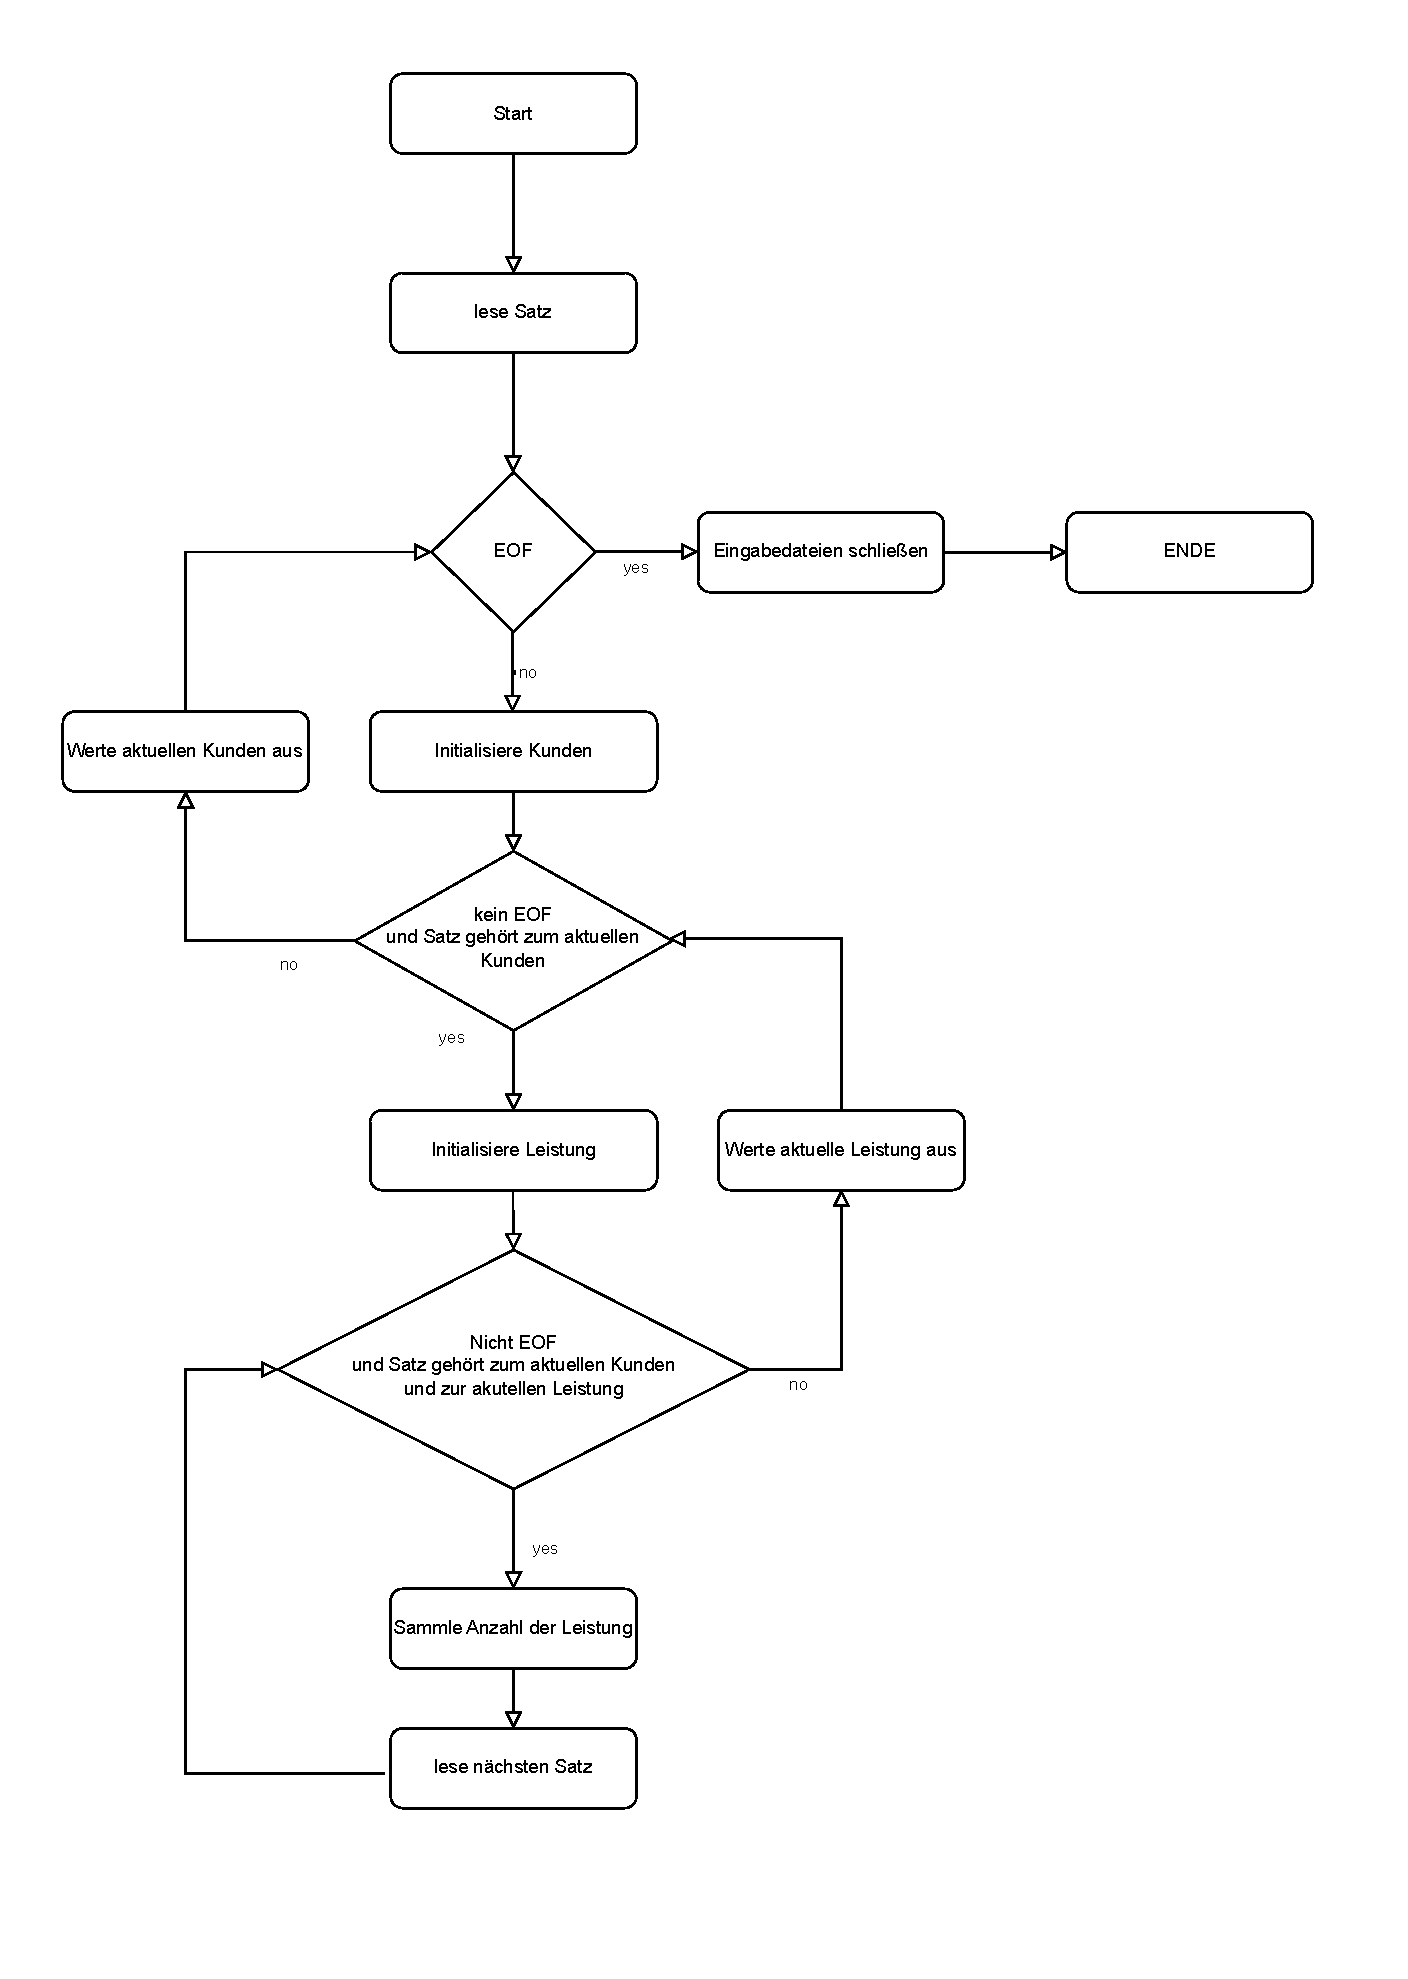
\includegraphics[scale=0.9,width=\textwidth,height=\textheight,keepaspectratio]{images/Gruppenwechsel-PAP.pdf}
    \caption{
        Veranschaulichung des Gruppenwechsels als Programmablaufplan
    }
    \label{fig:diagramm1}
\end{figure}

\begin{figure}[!h]
    \centering
    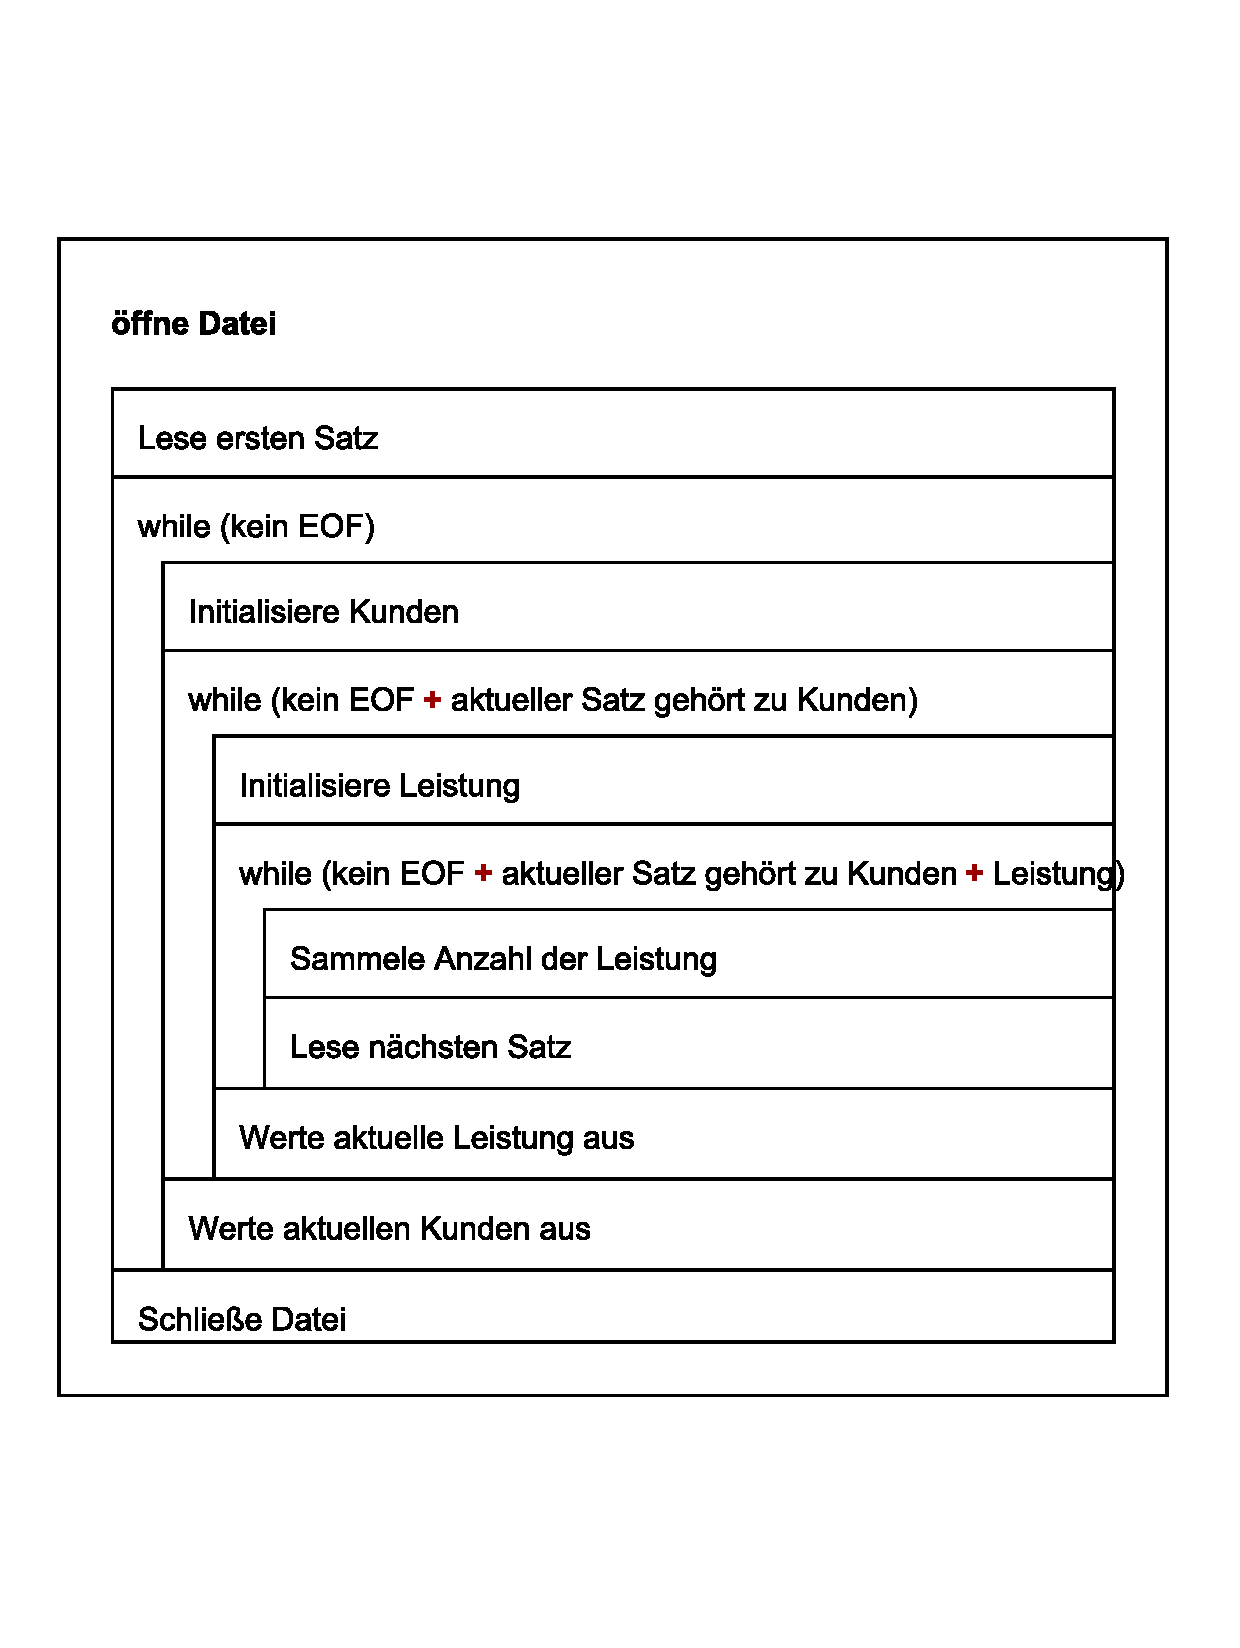
\includegraphics[width=\textwidth,height=\textheight,keepaspectratio]{images/Gruppenwechsel-NSD.pdf}
    \caption{
        Veranschaulichung des Gruppenwechsels als Nassi-Schneiderman-Diagramm
    }
    \label{fig:diagramm2}
\end{figure}

\begin{figure}[!h]
    \centering
    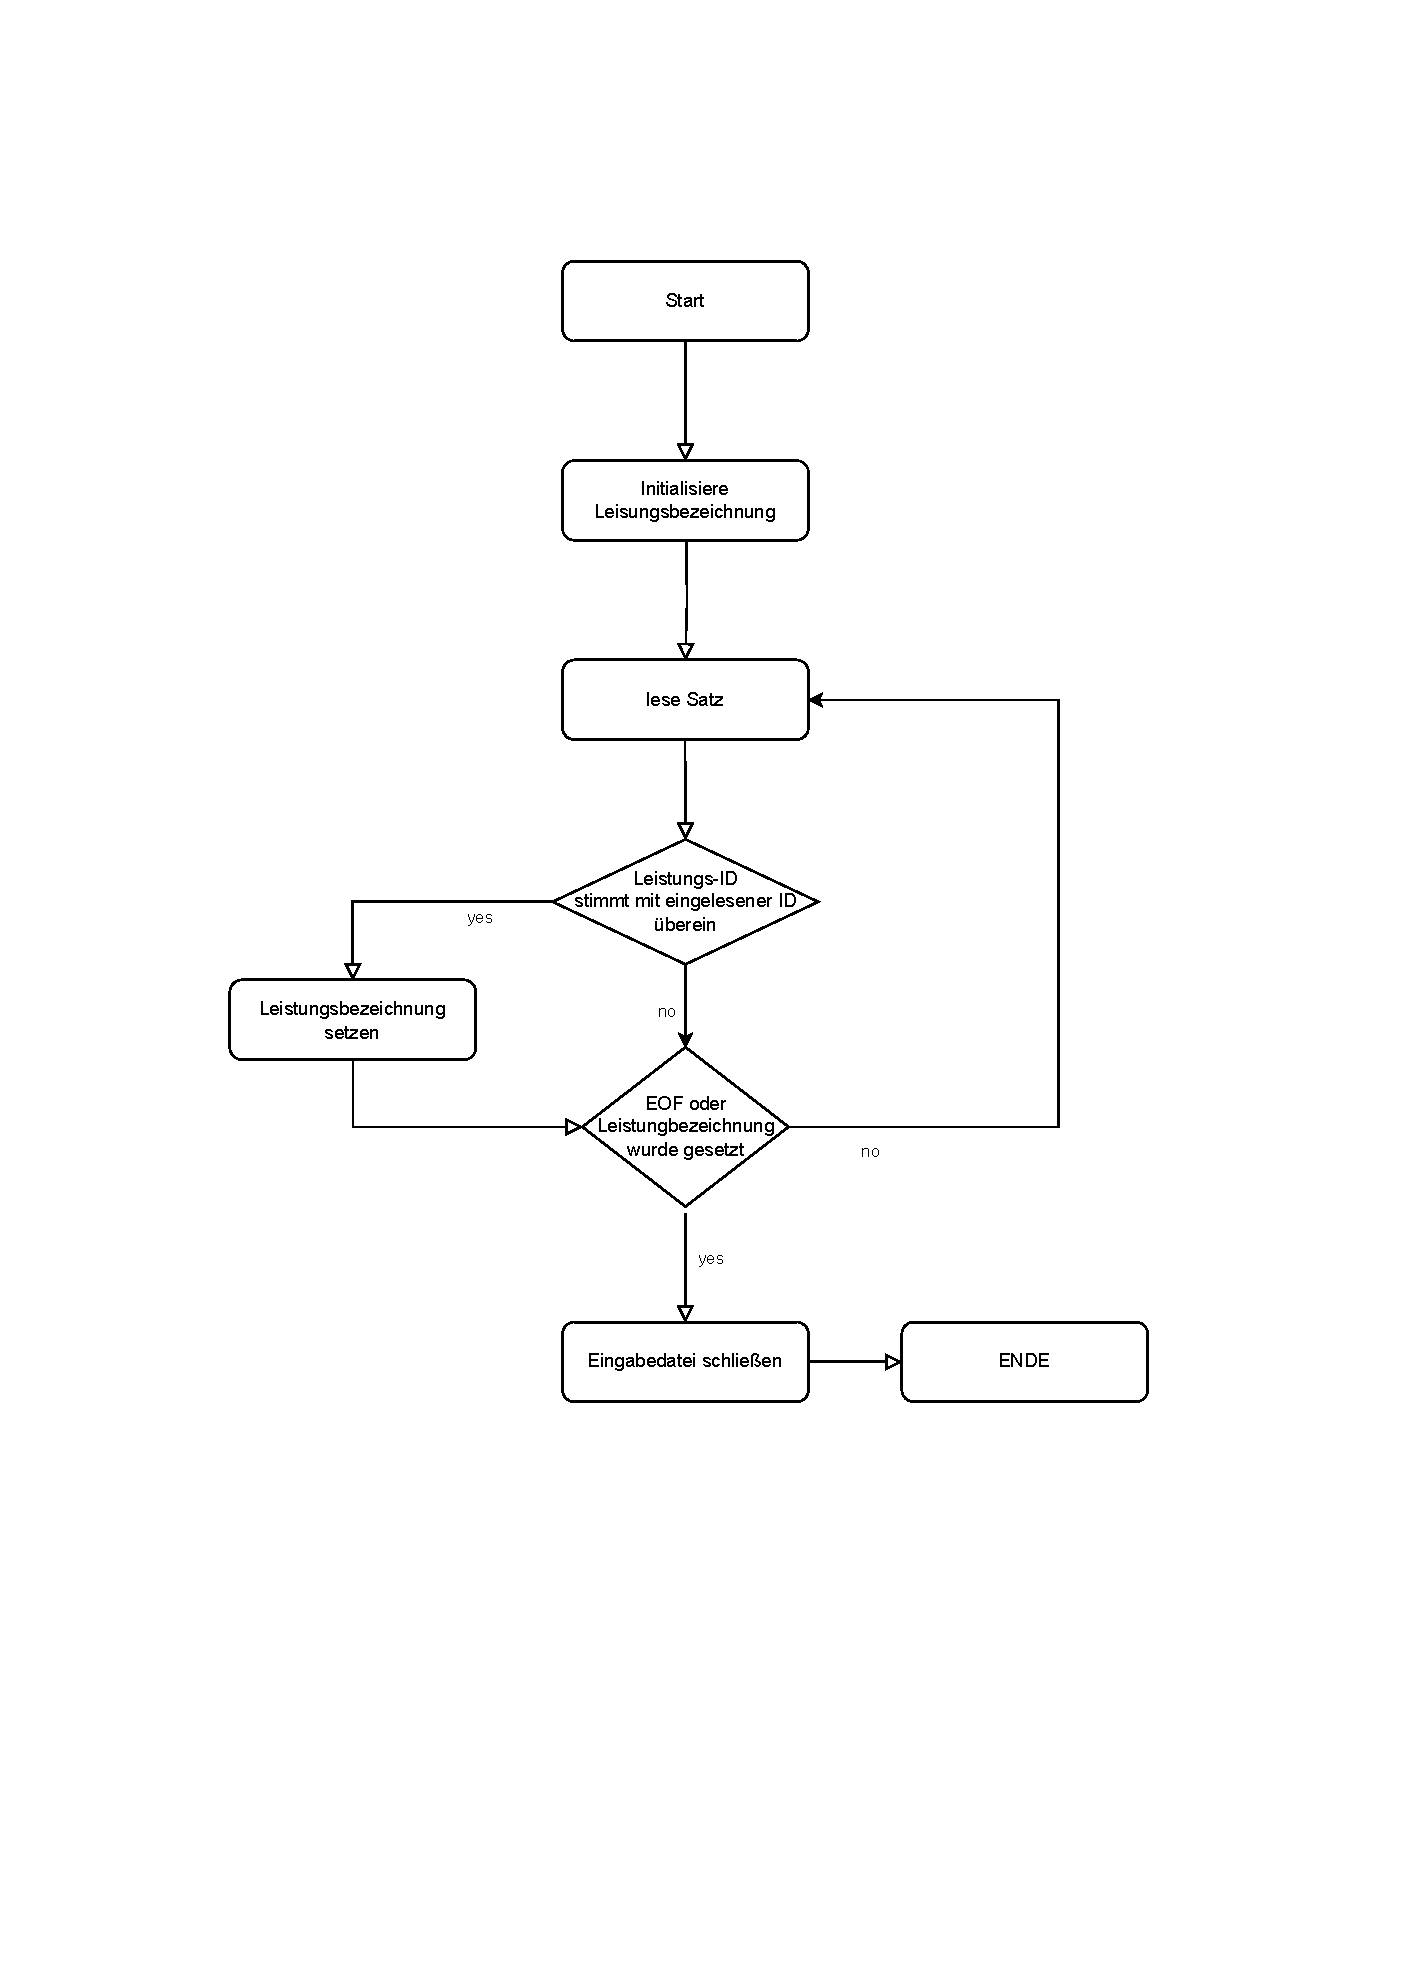
\includegraphics[width=\textwidth,height=\textheight,keepaspectratio]{images/Erhalte_Leistungsbezeichnung-PAP.pdf}
    \caption{
        Ablauf der Ermittlung der Leistungsbezeichnugnen
    }
    \label{fig:diagramm3}
\end{figure}



\section{Entwicklungsdokumentation}\label{sec:entwicklerdokumentation}
Es wurden grundsätzlich sprechende Namen für Variablen, Abschnitte und Paragrafen gewählt. Außerdem sind \texttt{DISPLAY} Statements welche zum Debuggen genutz wurden erhalten geblieben. Mit diesen ist der Programmablauf leichter nachzuvollziehen.

Die Funktionen der einzelnen Paragrafen sind in Tabelle~\ref{tab:prog-strukt} beschrieben.


\definecolor{fhfarbe}{HTML}{51B2AC}
\definecolor{fhfarbe2}{HTML}{4FAEAB}
\begin{table}[!htb]
    \centering
    \rowcolors{2}{black!5}{white}
    \begin{tabularx}{\textwidth}{X | X }
       \rowcolor{fhfarbe!25}
       Bezeichnung                             & Beschreibung             \\
%       \hline
       \rowcolor{fhfarbe!10}
       MAIN-PROCEDURE & Hauptablauf welcher den Gruppenwechsel delegiert \\
       PREPERATION & Spiegelt den Vorlauf zum einlesen einer Datei wieder und öffnet die Eingabe- (JOURNAL.txt) und Ausgabedatei (INVOICE.txt) \\
       CUSTOMER-PREPERATION & Wertet den akutellen Einabesatz aus und initialisiert daraus einen Kunden \\
       SERVICE-PREPERATION & Wertet den aktuellen Eingabesatz aus und initialisiert daraus eine Leistung \\
       INDIVIDUAL-PROCESSING & Wertet den aktuellen Eingabesatz aus und zählt die Anzahl einer Leistung hoch \\
       READ-NEXT-LINE & Liest, wenn möglich, die nächste Zeile des Jounrals ein \\
       SERVICE-COMPLETION & Wertet die aktuelle Leistung aus indem der Gesamtbetrag der Leistung berechnet und mit allen relevanten Leistungsdaten in die Rechnung geschrieben wird \\
       CUSTOMER-COMPLETION & Wertet den aktuellen Kunden aus indem der Gesamtbetrag des Kunden in die Rechnung geschrieben und ein Ende gekennzeichnet wird \\
       COMPLETION & schließt Einlese- und Auslesedatei \\
       
       \rowcolor{fhfarbe!10}
       GET-SERVICE-TERM & Ermittelt anhand der Leistungs-ID durch einlesen des Leistungsglossar die Leistungsbeschreibung \\
       CHECK-LINE & Überprüft, ob die aktuell aus dem Glossar eingelesene Leistungs-ID mit der zu überprüfenden Leistungs-ID übereinstimmt \\
       NEXT-LINE & Liest, wenn möglich die nächste Zeile des Glossars ein\\
       DISPLAY-JOURNAL & Debugeinheit zum ausgeben der aktuell eingelesenen Daten \\
    \end{tabularx}
    \caption{Aufgaben der einzelnen logischen Einheiten.}\label{tab:prog-strukt}
\end{table}

    \addtocontents{toc}{\protect\newpage}
    \chapter{Testdokumentation}\label{ch:testdokumentation}
Alle Testfälle können wie beschrieben in~\enquote{\nameref{sec:testen-der-beispiele}}~ausgeführt werden.
Für eine klare Struktur wurden Sie in 4 verschiedene Testgruppen eingeteilt:
\begin{enumerate}[label={\textbf{Gruppe~\arabic*:}}, ref={Gruppe~\arabic*}, leftmargin=*, noitemsep]
    \label{enm:tesgruppen}
    \item Tests, welche die Aufgabestellung wiederspiegeln.
    \item Allgemeine Testfälle.
    \item Überprüfungen der minimal Fälle.
    \item Sonderfall Testfälle.
\end{enumerate}

Die in der Aufgabenstellung definierten Tests werden im Folgenden ausführlich beschrieben.
Dabei werden die allgemeine Funktionalität des Programms getestet.

\section{Aufgabenstellung}\label{subsec:aufgabenstellung}
\begin{figure}[!h]
    \centering
    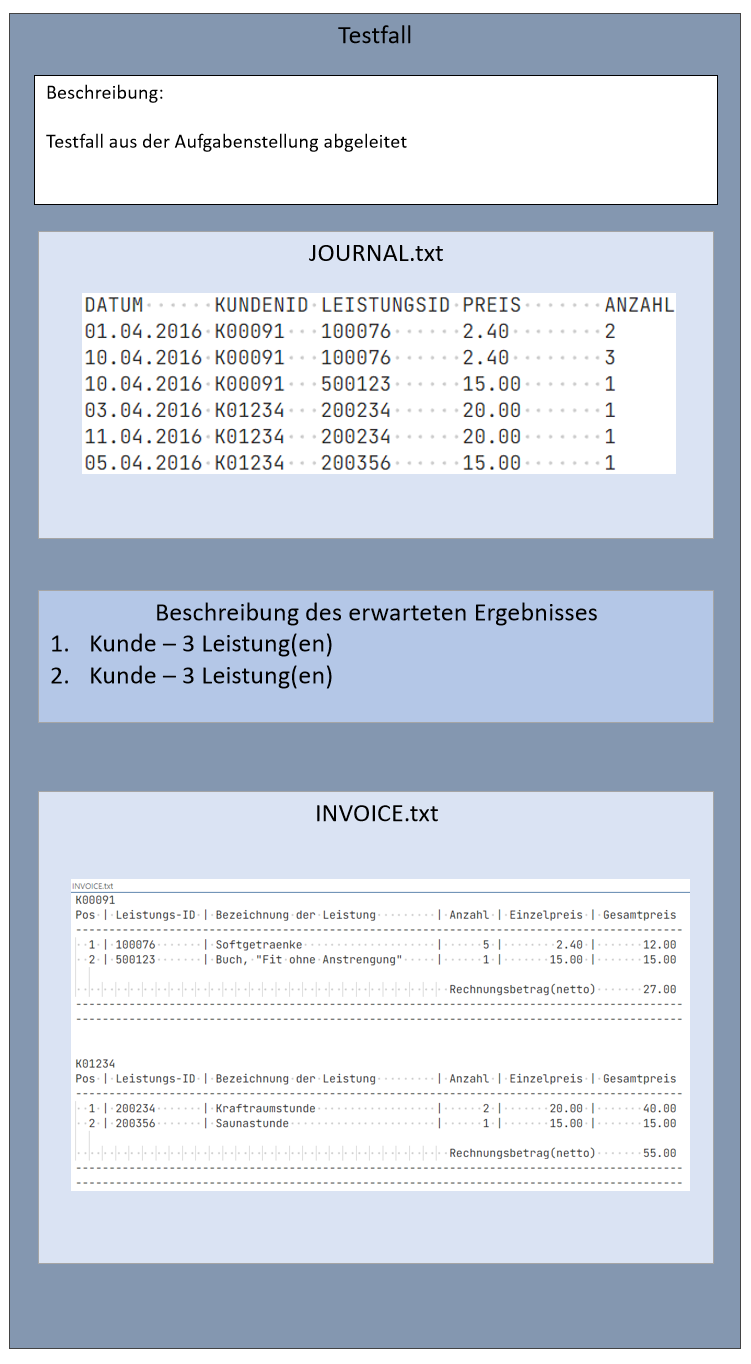
\includegraphics[width=\textwidth,height=\textheight,keepaspectratio]{images/Testdokumentation/Aufgabestellung/aufgabenstellung.png}
    \caption{Aufgabenstellung}
\end{figure}

\section{Allgemeine Tests}\label{sec:allgemeine-tests}
\begin{figure}[!h]
    \centering
    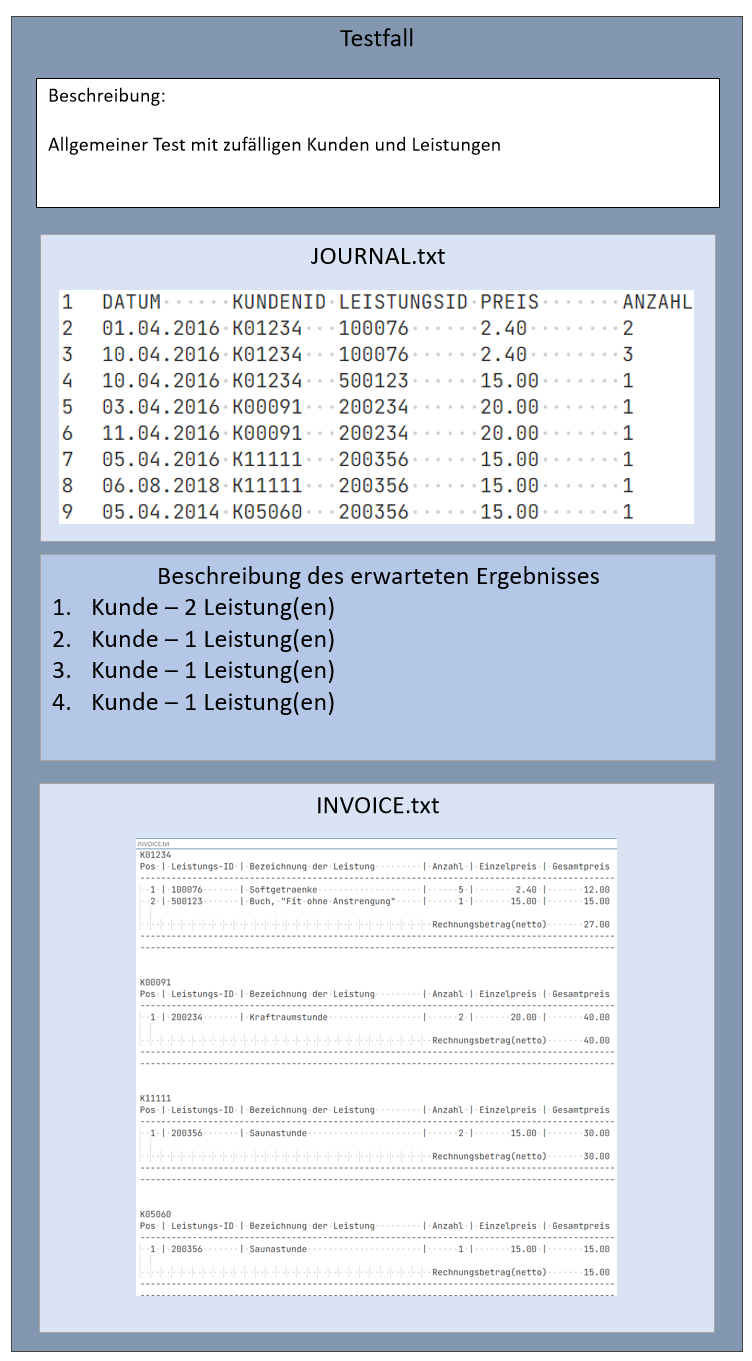
\includegraphics[width=\textwidth,height=\textheight,keepaspectratio]{images/Testdokumentation/Allgemeinfälle/fall_1.png}
    \caption{Allgemeiner Testfall 1}
\end{figure}

\begin{figure}[!h]
    \centering
    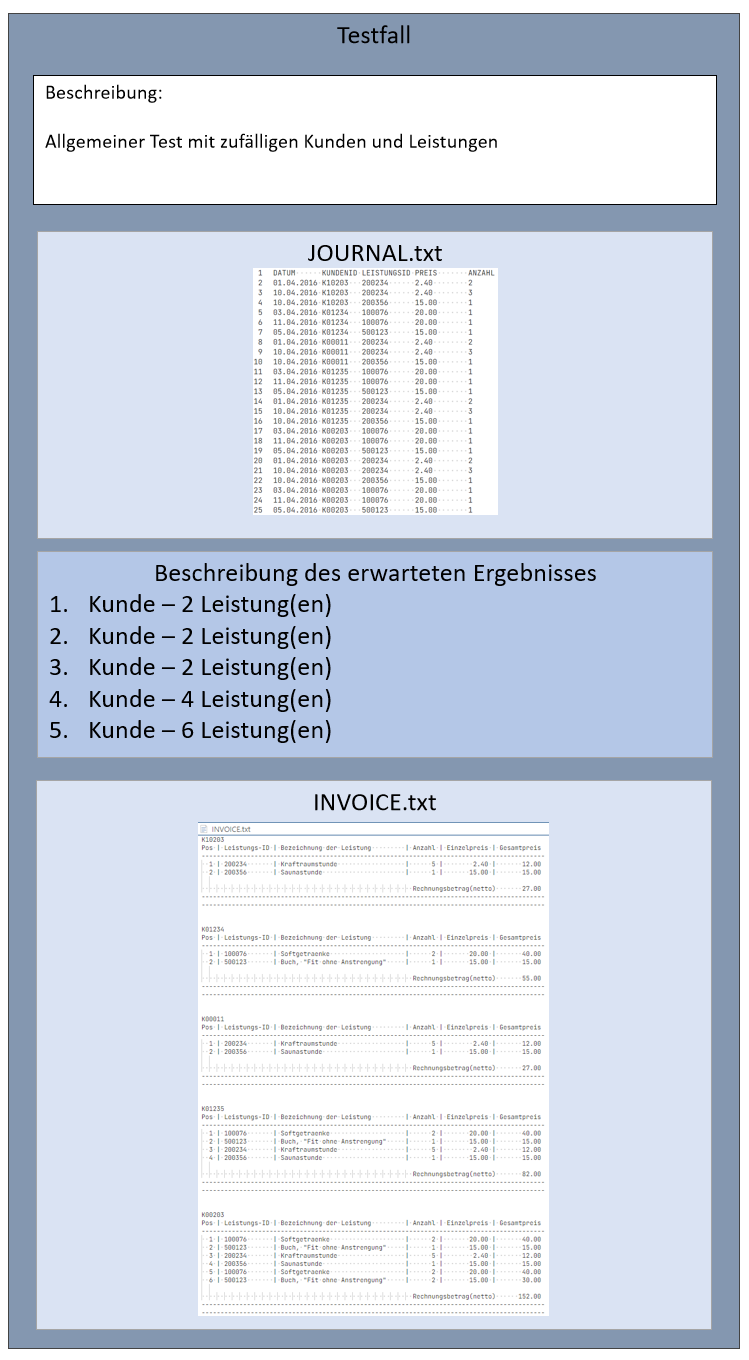
\includegraphics[width=\textwidth,height=\textheight,keepaspectratio]{images/Testdokumentation/Allgemeinfälle/fall_2.png}
    \caption{Allgemeiner Testfall 2}
\end{figure}

\begin{figure}[!h]
    \centering
    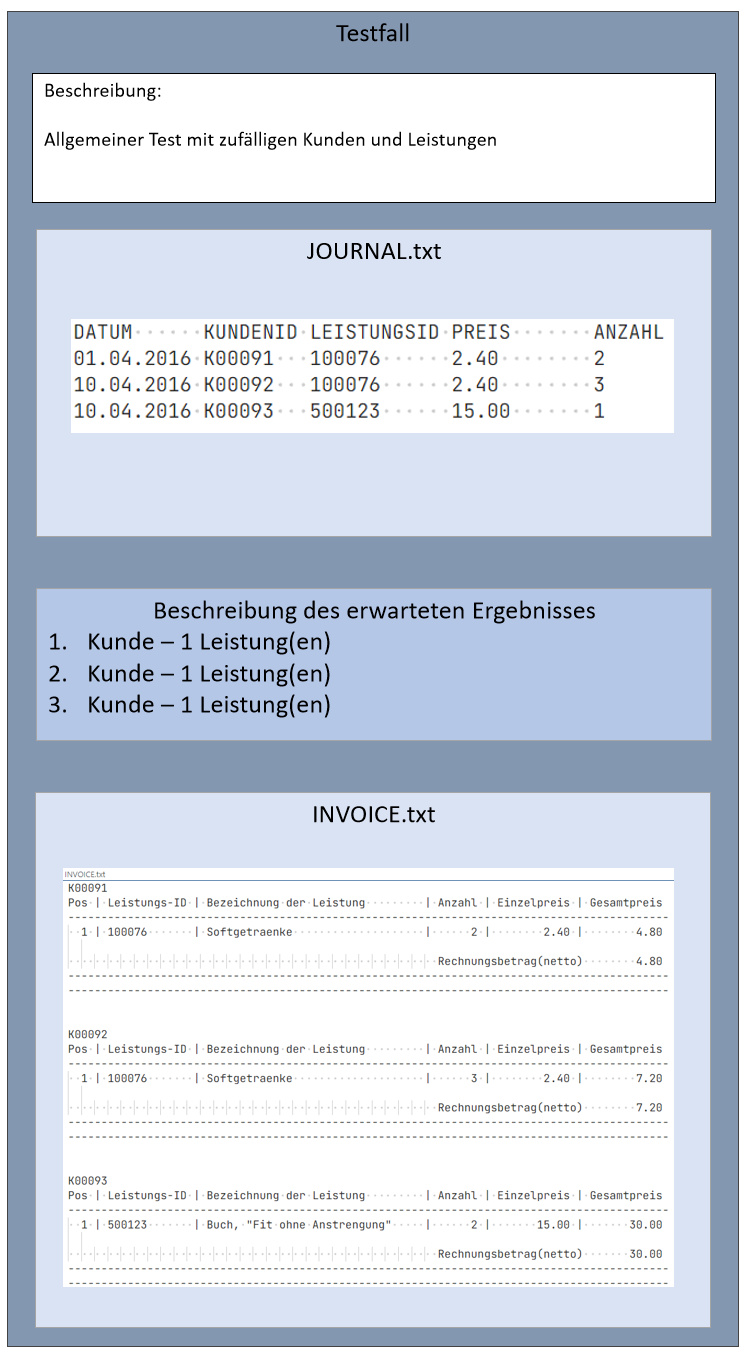
\includegraphics[width=\textwidth,height=\textheight,keepaspectratio]{images/Testdokumentation/Allgemeinfälle/fall_3.png}
    \caption{Allgemeiner Testfall 3}
\end{figure}

\section{Minimalfälle}\label{sec:minimalfaelle}
\begin{figure}[!h]
    \centering
    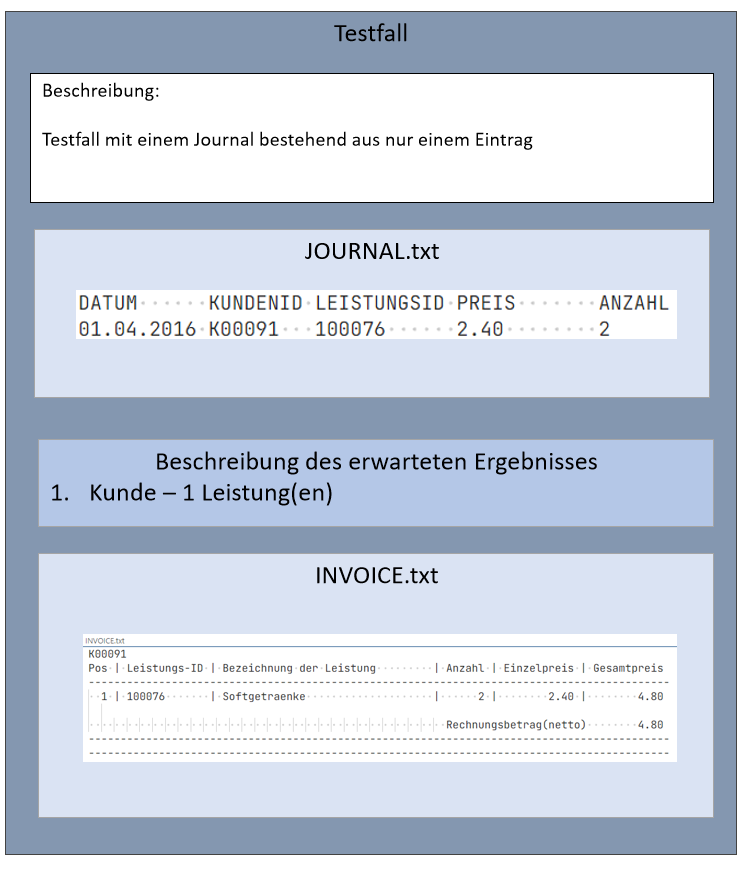
\includegraphics[width=\textwidth,height=\textheight,keepaspectratio]{images/Testdokumentation/Minimalfälle/1_eintrag.png}
    \caption{Journal mit nur einem Eintrag}
\end{figure}

\begin{figure}[!h]
    \centering
    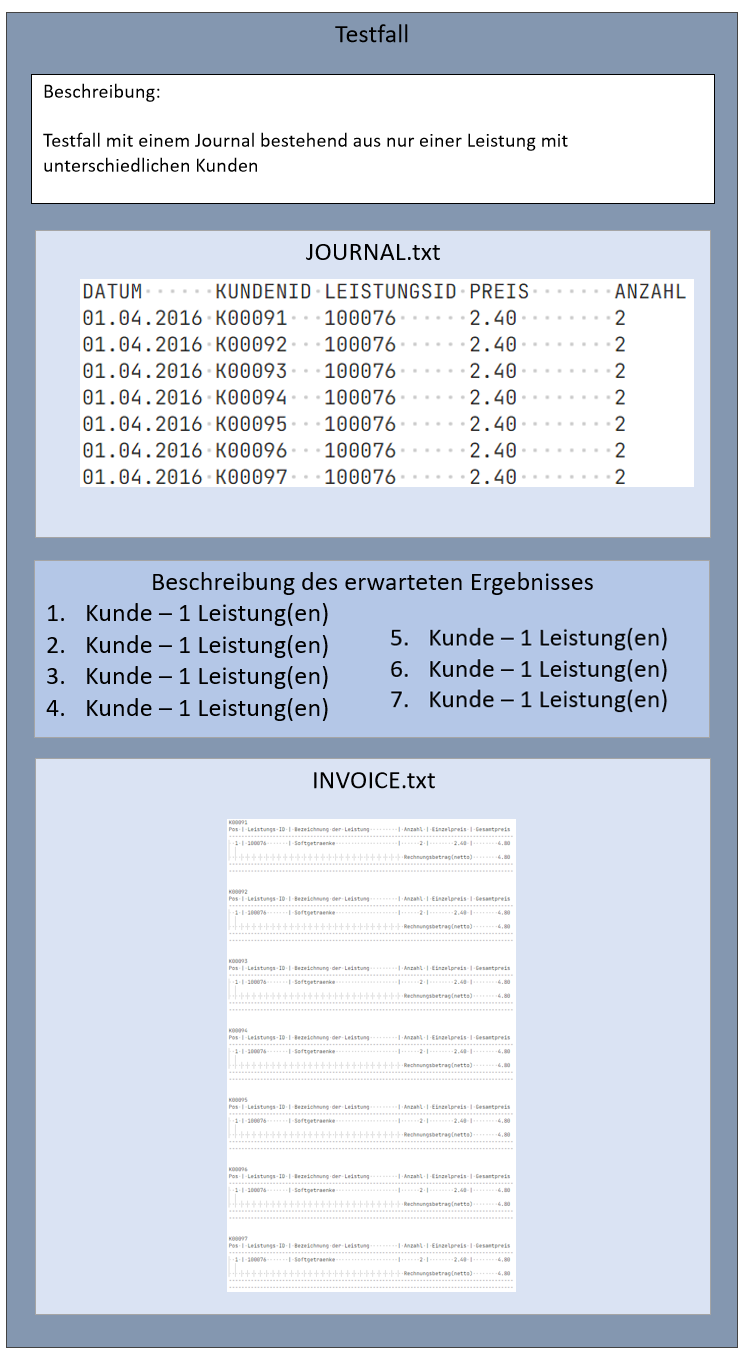
\includegraphics[width=\textwidth,height=\textheight,keepaspectratio]{images/Testdokumentation/Minimalfälle/1_kunde_verschiedene_leistungen.png}
    \caption{Journal mit nur einem einzigen Kunden}
\end{figure}

\begin{figure}[!h]
    \centering
    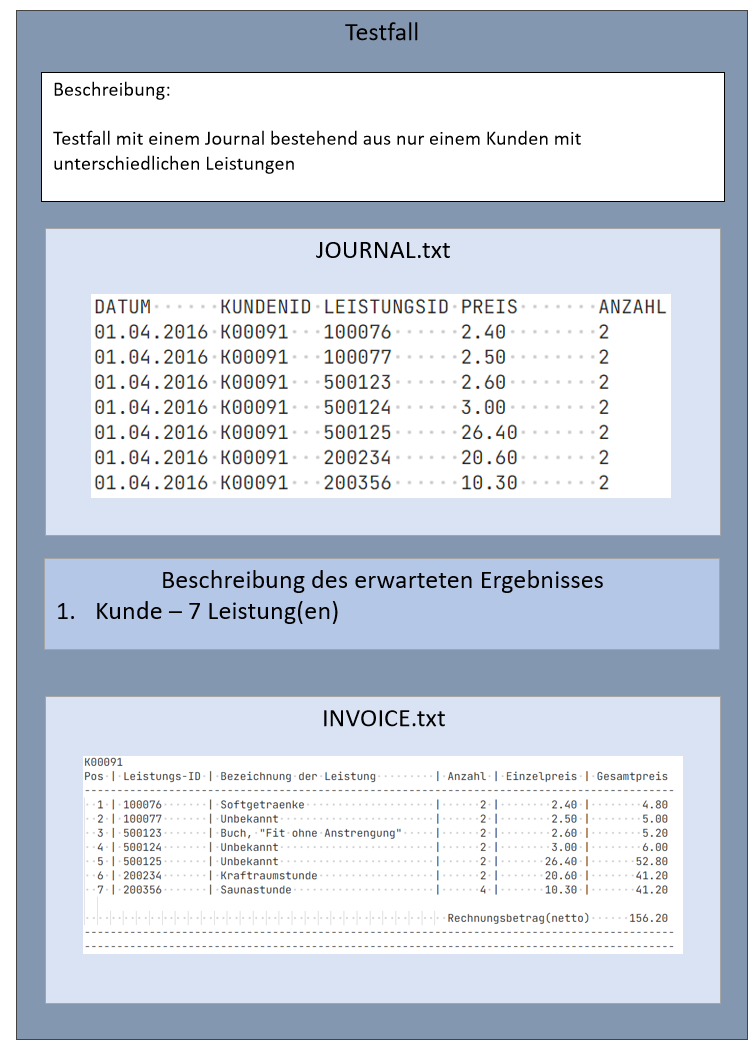
\includegraphics[width=\textwidth,height=\textheight,keepaspectratio]{images/Testdokumentation/Minimalfälle/verschiedene_kunden_1_leistung.png}
    \caption{Journal mit nur einer einzigen Leistung}
\end{figure}

\section{Sonderfälle}\label{sec:minimalfaelle}

\begin{figure}[!h]
    \centering
    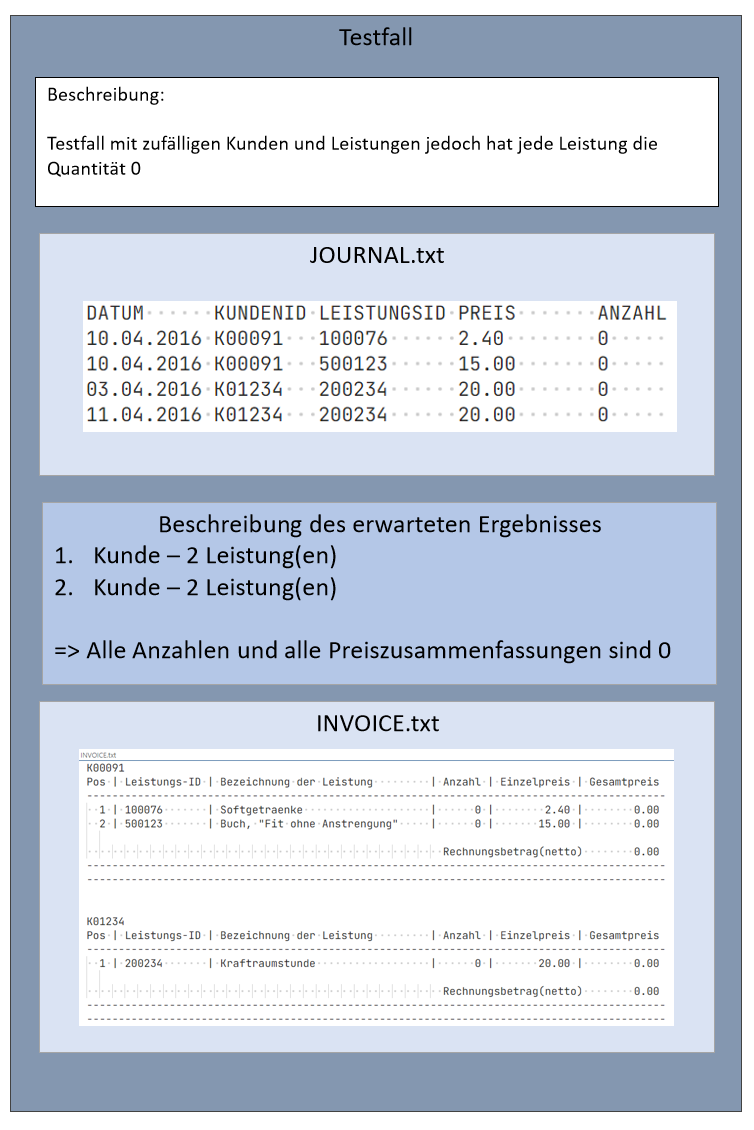
\includegraphics[width=\textwidth,height=\textheight,keepaspectratio]{images/Testdokumentation/Sonderfälle/anzahl_0.png}
    \caption{Alle Leistungen mit Anzahl 0}
\end{figure}

\begin{figure}[!h]
    \centering
    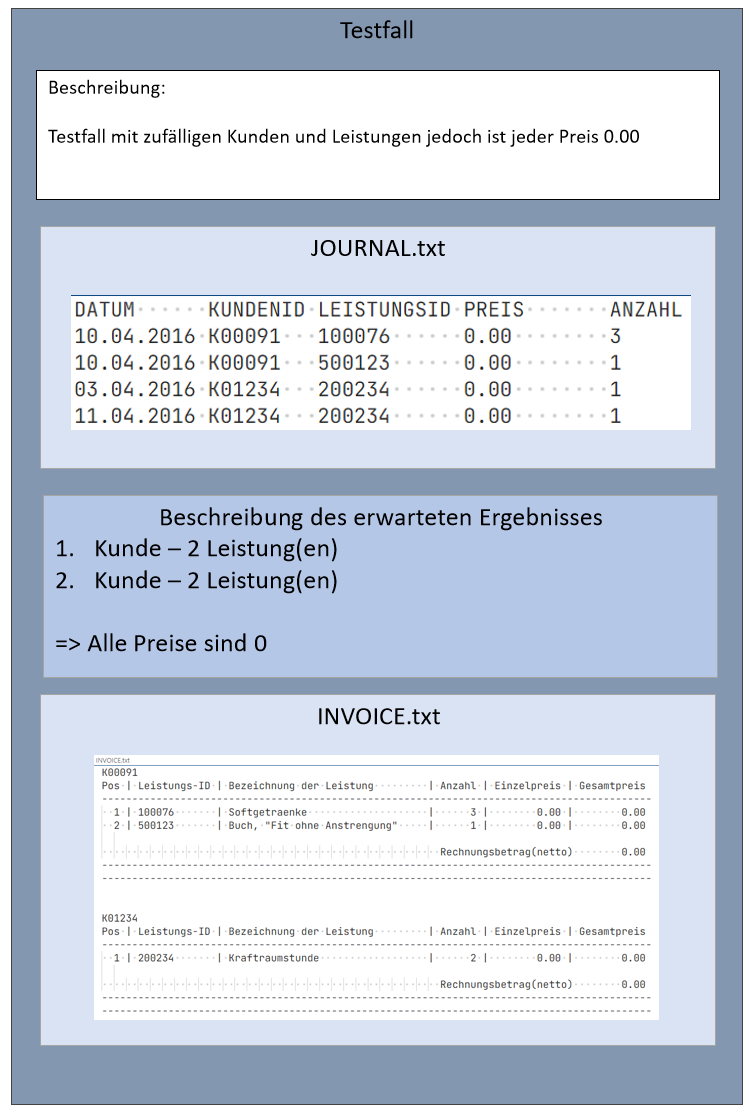
\includegraphics[width=\textwidth,height=\textheight,keepaspectratio]{images/Testdokumentation/Sonderfälle/preis_0.png}
    \caption{Alle Leistungen mit Preis 0.00}
\end{figure}

\begin{figure}[!h]
    \centering
    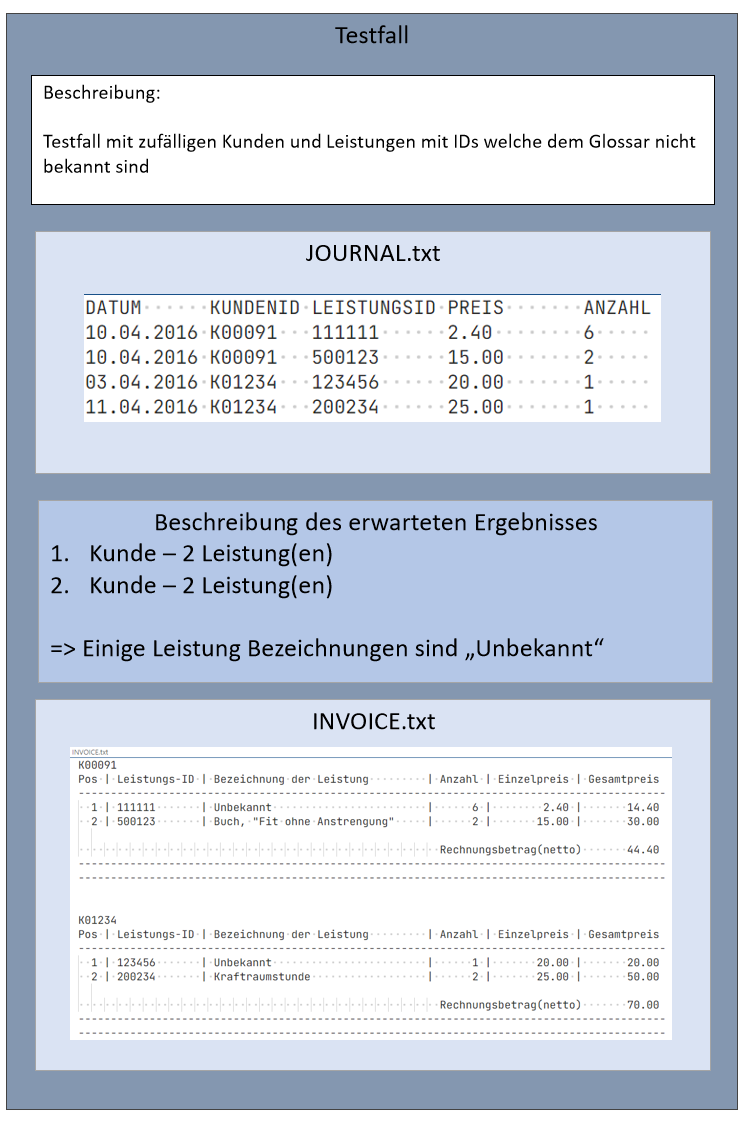
\includegraphics[width=\textwidth,height=\textheight,keepaspectratio]{images/Testdokumentation/Sonderfälle/unbekannte_leistung.png}
    \caption{Leistung-IDs sind teilweise nicht im Glossar vorhanden}
\end{figure}
    \chapter{Zusammenfassung und Ausblick}\label{ch:zusammenfassung-und-ausblick}


\section{Zusammenfassung}\label{sec:zusammenfassung}
Es wurde eine Software angefertigt, welche alle Vorgaben bezüglich der geforderten Funktionalität erfüllt.
Der gesamte Ablauf, vom Einlesen eines externen Wörterbuchs, über das eigentliche Mapping der Tasten und der Datenstruktur, bis hin zur Behandlung von Fehlerfällen und das Schreiben eines neuen Wörterbuchs, wurde korrekt abgebildet.\\

Mithilfe dieser Entwicklung können vereinfacht Texteingaben auf Tastaturen mit gleichem Aufbau, wie die eines Mobiltelefons, getätigt werden.\\
Bei der Implementierung wurde stets darauf geachtet, die Modularisierung einzuhalten, um mögliche Erweiterungen einfach einbinden zu können.
Eine ausführliche Test- und Entwicklungsdokumentation und ein Programmablaufplan geben projektfremden Personen, besonders Entwicklern einen tiefen Einblick in die Software und ihrer Funktionsweise.
Weitergehend wurden sprechende Variablennamen mit Namenskonventionen gewählt, um die Wartbarkeit des Codes maximal zu halten.


\section{Ausblick}\label{sec:ausblick}
Die entwickelte Software kann vielseitig erweitert und verbessert werden.

Eine mögliche Verbesserung wäre eine striktere Kontrolle der externen Wörterbücher.
Aktuell werden die Dateien nur minimal auf syntaktische Anforderungen überprüft, der Inhalt der einzelnen Zeilen wird aber nicht validiert.

Des Weiteren könnte die größe des internen Wörterbuchs dynamische zur Laufzeit erweitert werden.
Im Moment gibt es eine feste maximale Größe, sodass das Wörterbuch irgendwann voll ist.
Die Tabellenstrukturen liegen dafür schon in der passenden Form vor.

Auch Programmausgaben im Benutzerdialog haben Verbesserungspotential.
Alle eingegebenen Sätze könnten zum Beispiel als Paragraf am Programmende ausgegeben werden.

Zudem könnte ein noch größerer Fokus auf COBOL-Code-Konventionen gelegt werden.

    % ============= Buchstabenteil ==============
    \renewcommand{\thechapter}{\Alph{chapter}}%
    \setcounter{chapter}{0}
%    \chapter{Abweichung und Ergänzung}\label{ch:abweichung-und-ergaenzung}
Die originale Planung wurde, mit Ausnahme von ein paar kleinen Änderungen, eingehalten.
    \chapter{Benutzeranleitung}\label{ch:benutzeranleitung}


\section{Vorbereiten des Systems}\label{sec:vorbereiten-des-systems}

\subsection{Systemvoraussetzungen}\label{subsec:systemvoraussetzungen}
Um das Programm zu benutzen ist ein Windows- oder Linux-System vorausgesetzt.
Unter Linux muss zusätzlich \textit{Wine}~installiert werden.

\subsection{Installation}\label{subsec:installation}
Die Installation des Programms erfolgt über das Entpacken der~.zip-Datei.
Die ausführbare .exe befindet sich im Anschluss im Unterordner \textit{bin}.
Außerdem ist es notwendig, dass unter Windows die PATH-Variable den Pfad zu GnuCOBOL/bin enthält.

\section{Programmaufruf}\label{sec:programmaufruf}
Um das Programm zu starten, muss die bin/TexteingabeHandy.exe aufgerufen werden.
Es öffnet sich ein Dialogfenster, mit welchem der Nutzer anschließend interagieren kann.


\section{Testen der Beispiele}\label{sec:testen-der-beispiele}
Die Beispiele können alle mittels der~.cmd-Dateien im bin Verzeichnis getestet werden.
Die TestAll.cmd enthält dabei alle Testfälle, welche automatisch nacheinander ausgeführt werden.
Hilfreich ist es, die ScreenBuffer-Size der Eingabeaufforderung auf eine höhere Zahl zu setzen, damit alle Zeilen in dem Dialogfenster bestehen bleiben.
Zu empfehlen ist hierbei eine Zahl über 1000.
    \chapter{Entwicklungsumgebung}\label{ch:entwicklungsumgebung}

Das Programm wurde mithilfe der OpenCobolIDE (\url{https://launchpad.net/cobcide/+download}) in der Version 4.7.6 geschrieben.
Dabei handelt es sich um eine leichtgewichtige COBOL Entwicklungsumgebung, die als Compiler GnuCOBOL 2.0.0 (\url{https://sourceforge.net/projects/gnucobol/}) verwendet.

Im Entwicklungsprozess wurde zur Versionsverwaltung GitHub (\url{https://github.com/}) verwendet.
Die dort angebotenen Remote-Repositories ermöglichen eine Versionierung und Backups des Quellcodes.

Alle Entwicklungsschritte wurden auf Systemen mit Windows 10 Betriebssystem (\url{https://www.microsoft.com/de-de/software-download/windows10}) durchgeführt.

\begin{figure}[htb]
    \centering
    \begin{minipage}{.5\textwidth}
        \centering
        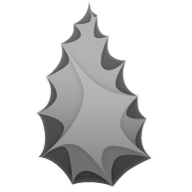
\includegraphics[width=.4\linewidth]{images/opencobol-logo}
    \end{minipage}%
    \begin{minipage}{.5\textwidth}
        \centering
        
\includegraphics[width=.4\linewidth]{images/Gnu-COBOL}
    \end{minipage}
    \caption{Logos von OpenCobolIDE und GnuCOBOL.}
    \label{fig:cobol-logos}
\end{figure}

\begin{figure}[htb]
    \centering
    
\includegraphics[width=.15\linewidth]{images/GitHub-Logo}
    \caption{
        GitHub-Logo.
    }
    \label{fig:github}
\end{figure}

    \chapter{Verwendete Hilfsmittel}\label{ch:verwendete-hilfsmittel}

Als Hilfsmittel wurden hauptsächlich die Inhalte der, von Prof. Dr. rer. nat. Karola Merkel (\url{https://www.fh-aachen.de/fachbereiche/medizintechnik-und-technomathematik/einrichtungen/sp-studienort-koeln/kontakt}) angebotenen, Vorlesung \glqq COBOL\grqq{} verwendet.
Zudem konnten unterschiedliche Fragen durch das Durchsuchen von Foren gelöst werden.
Besonders häufig konnte das \glqq Expertforum \glqq stackoverflow\grqq{} (\url{stackoverflow.com}) Antworten liefern.
    \chapter{Erklärung}\label{ch:erklaerung}

Hiermit versichere ich, dass ich die vorliegende Arbeit mit dem Thema
\begin{quote}
    \textit{\titleDocument}
\end{quote}
selbstständig verfasst und keine anderen als die angegebenen Quellen und Hilfsmittel benutzt habe.
Alle Ausführungen, die anderen Schriften wörtlich oder sinngemäß entnommen wurden, sind kenntlich gemacht und die Arbeit ist in gleicher oder ähnlicher Fassung noch nicht Bestandteil einer Studien- oder Prüfungsleistung.
\\

\vspace*{2cm}

\begingroup
\setlength{\parindent}{0pt} % keine Einrückung bei neuen Absätzen in diesem Bereich

\locationDocument, den \dateDocument
\bigskip
\bigskip

% gewünschte Breite der Unterschriftslinie
\newlength{\widthbox}
\settowidth{\widthbox}{\locationDocument, den \dateDocument}

\makebox[\widthbox]{\hrulefill}\\
\authorDocument
\endgroup
\newpage

    \chapter{Aufgabenstellung}\label{ch:aufgabenstellung}

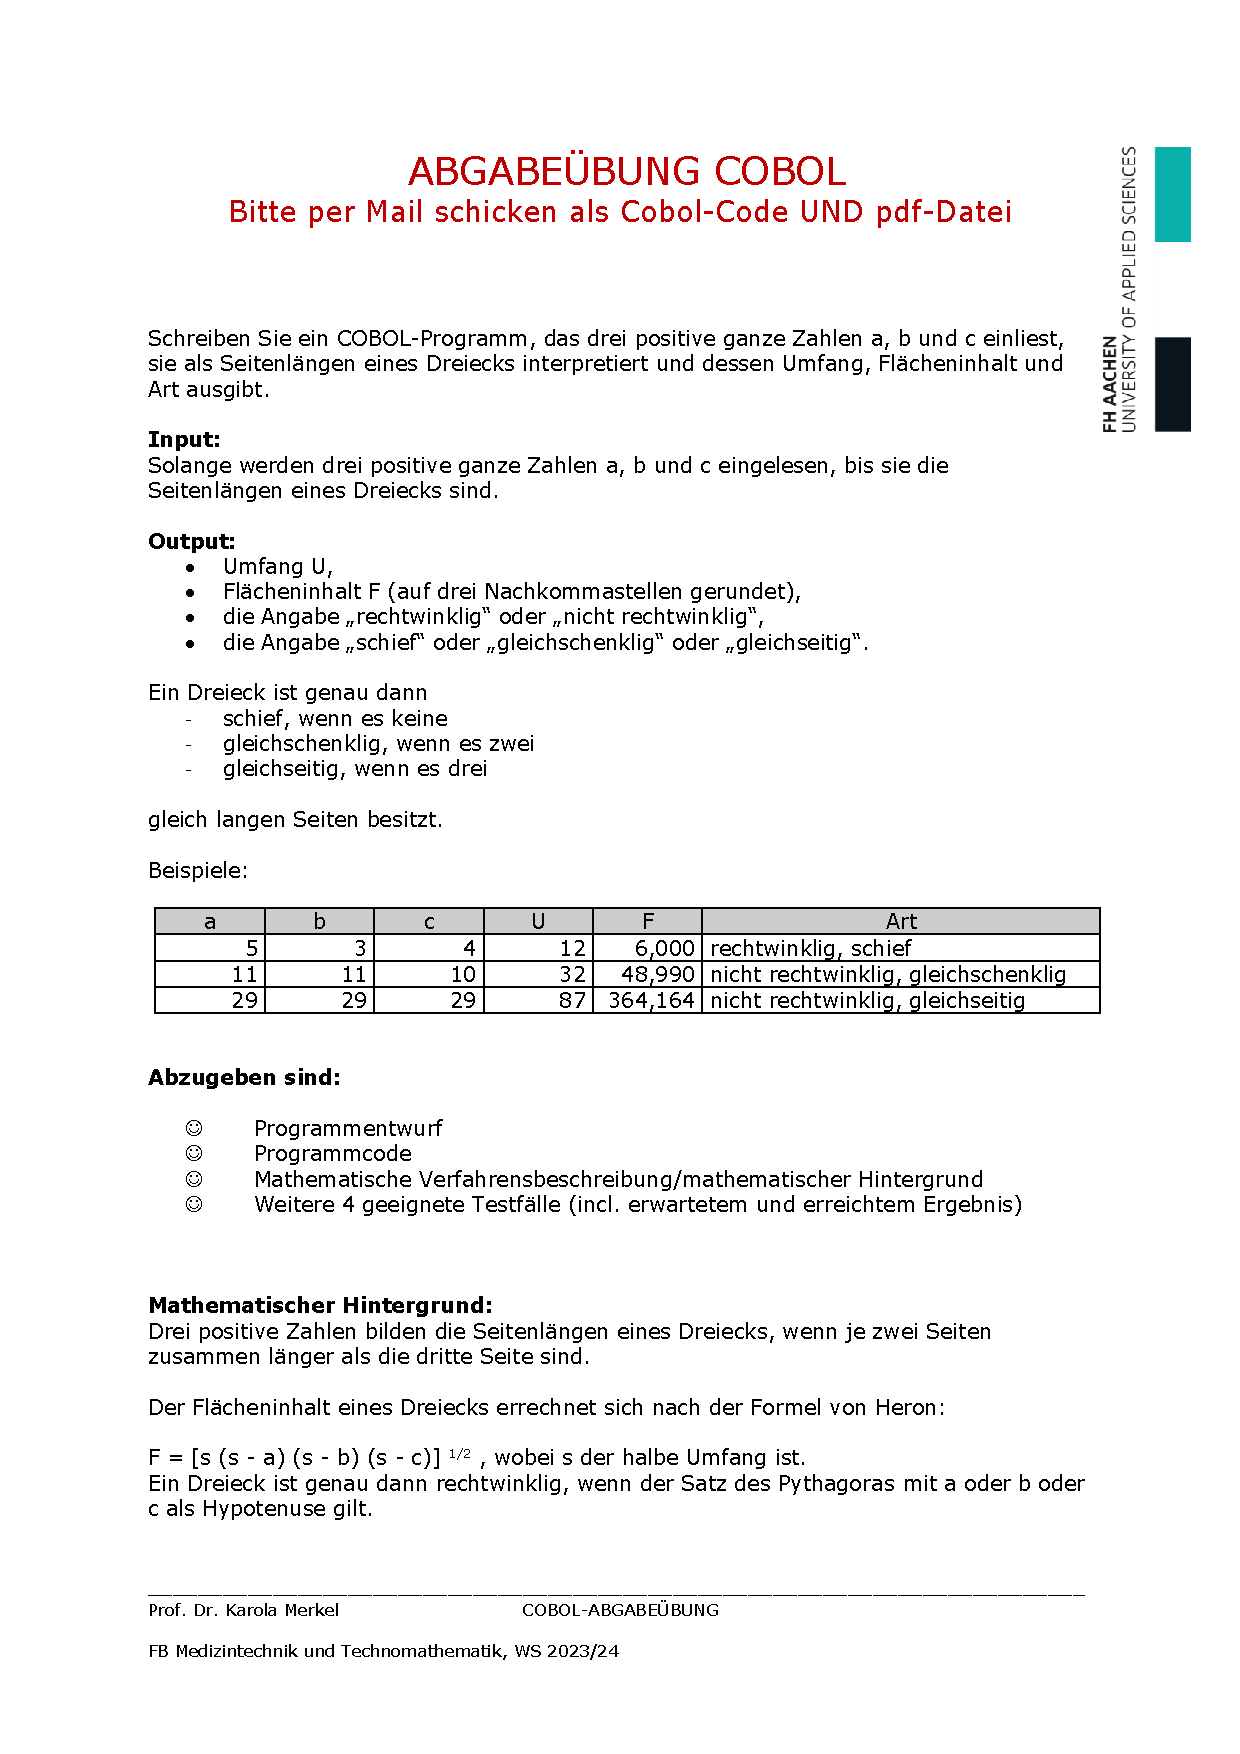
\includepdf[pages=-]{images/ABGABEUEBUNG 2023_23.pdf}
    \chapter{Quellcode}\label{ch:quellcode}
\end{document}
